\documentclass[..thesis.tex]{subfiles}

\usetikzlibrary{3d}
\usetikzlibrary{patterns}

\tikzset{xyp/.style={canvas is xy plane at z=#1}}
\tikzset{xzp/.style={canvas is xz plane at y=#1}}
\tikzset{yzp/.style={canvas is yz plane at x=#1}}


\begin{document}

\toguide{Okay, what's next?}

The key challenge for Goblint is the number of false-positives. It is clear that even if one can guarantee the soundness of the 
underlying analysis, then there is a threshold of incorrect warnings above what the results of the analysis contain too much noice
to be of help for a programmer.

\toguide{I buy it, what can be done about it?}

One of the steps taken to reduce the the number of false-positives is the usage of \textit{happen-before} relation.

\toguide{How can you use happen-before here?}

Consider following device driver:

\begin{lstlisting}[language=c,style=def]

static int i = 0;

static int file_open(...)
{
    printk( "Opening device \n");
    return 0;
}

static int file_open(...)
{
    printk( "Opening device \n");
    return 0;
}

struct file_operations f_ops = {
  .open    = file_open,
  .release = file_close,
};

int init(...)
{
  publish_file_operations(f_ops);
  i += 1;
  return 0;
}

int exit(...)
{
  i -= 1;
  return 0;
}

\end{lstlisting}

As mentioned previously, \textit{init} and \textit{exit} functions are used by kernel register and de-register a device. As after publishing the file operations, Goblint cannot assume that the functions of the driver are called by one thread, a possible data-race is detected between the operations on variable $i$ in functions \textit{init} and \textit{exit}. At same time, the Linux Kernel does not allow a call to the \textit{exit} function until the call to the \textit{init} function is called and all the opened files are released.

We would like to have Goblin know about that guarantee and make use of the information that the call to \textit{init} will always complete before call to \textit{exit}.

\toguide{Example makes sense, but how to practically make use of it?}

To do so, we extend the region based analysis of Goblint.

\begin{figure}[H]
  \centering
    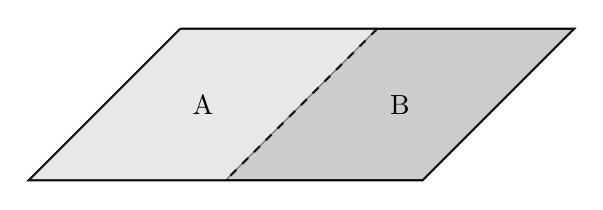
\begin{tikzpicture}
      \pgfmathsetmacro{\cubex}{5}
      \pgfmathsetmacro{\cubey}{5}
      \pgfmathsetmacro{\cubez}{5}
      \draw[thick,-] (0,0,0) -- ++(\cubex,0,0) -- ++(0,0,\cubez) -- ++(-\cubex,0,0) --  ++(0,0,-\cubez);
      \draw[thick,dashed] (2.5,0,0) -- (2.5,0,5);
      \fill[opacity=0.3,black!30,draw=black,xzp=0] (0,0) rectangle (2.5,5);
      \fill[opacity=0.3,black!65,,draw=black,xzp=0] (2.5,0) rectangle (5,5);
      \node at (0.25*\cubex,0,2.5) (A) {A};
      \node at (0.75*\cubex,0,2.5) (B) {B};
    \end{tikzpicture}
\end{figure}

\begin{figure}[H]
  \centering
    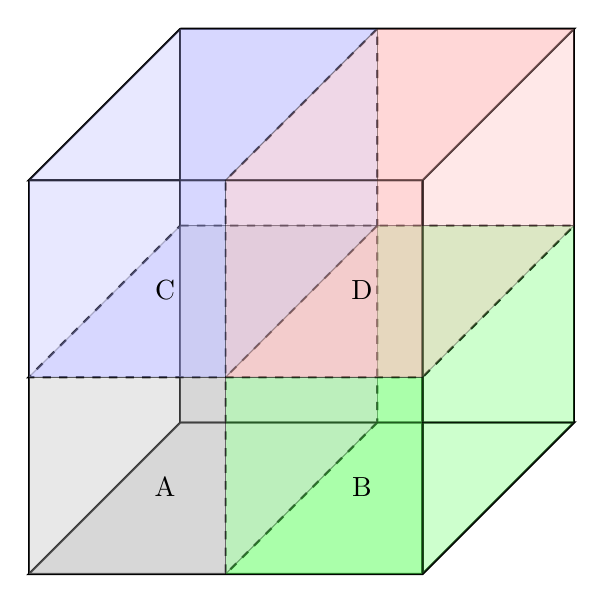
\begin{tikzpicture}
      \pgfmathsetmacro{\cubex}{5}
      \pgfmathsetmacro{\cubey}{5}
      \pgfmathsetmacro{\cubez}{5}
      \draw[thick,-] (0,0,0) -- ++(\cubex,0,0) -- ++(0,0,\cubez) -- ++(-\cubex,0,0) --  ++(0,0,-\cubez);
      \draw[thick,-] (0,\cubey,0) -- ++(\cubex,0,0) -- ++(0,0,\cubez) -- ++(-\cubex,0,0) --  ++(0,0,-\cubez);
      \draw[thick,dashed] (0,0.5*\cubey,0) -- ++(\cubex,0,0) -- ++(0,0,\cubez) -- ++(-\cubex,0,0) --  ++(0,0,-\cubez);
      \draw[thick,-] (0,0,0) -- (0,\cubey,0);
      \draw[thick,-] (\cubex,0,0) -- (\cubex,\cubey,0);
      \draw[thick,-] (\cubex,0,\cubez) -- (\cubex,\cubey,\cubez);
      \draw[thick,-] (0,0,\cubez) -- (0,\cubey,\cubez);
      
      \draw[thick,dashed] (0.5*\cubex,0,0) -- ++(0,0,\cubez) -- ++(0,\cubey,0) -- ++(0,0,-\cubez) -- ++(0,-\cubey,0);
      \draw[thick,dashed] (0.5*\cubex,0.5*\cubey,0) -- ++(0,0,\cubez); 

      \fill[opacity=0.3,black!30,draw=black,xzp=0] (0,0) rectangle (0.5*\cubex,\cubez);
      \fill[opacity=0.3,black!30,draw=black,xyp=0] (0,0) rectangle (0.5*\cubex,0.5*\cubey);
      \fill[opacity=0.3,black!30,draw=black,xyp=\cubez] (0,0) rectangle (0.5*\cubex,0.5*\cubey);

      \fill[opacity=0.3,blue!30,draw=black,xzp=\cubez] (0,0) rectangle (2.5,5);
      \fill[opacity=0.3,blue!30,draw=black,xzp=0.5*\cubez] (0,0) rectangle (2.5,5);
      \fill[opacity=0.3,blue!30,draw=black,xyp=0] (0,0.5*\cubey) rectangle ++(0.5*\cubex,0.5*\cubey);
      \fill[opacity=0.3,blue!30,draw=black,xyp=\cubez] (0,0.5*\cubey) rectangle ++(0.5*\cubex,0.5*\cubey);

      \fill[opacity=0.3,green!65,draw=black,xzp=0] (2.5,0) rectangle (\cubex,\cubez);
      \fill[opacity=0.3,green!65,draw=black,xyp=0] (0.5*\cubex,0) rectangle ++(0.5*\cubex,0.5*\cubey);
      \fill[opacity=0.3,green!65,draw=black,xyp=\cubez] (0.5*\cubex,0) rectangle ++(0.5*\cubex,0.5*\cubey);

      \fill[opacity=0.3,red!30,draw=black,xzp=\cubey] (2.5,0) rectangle (\cubex,\cubez);
      \fill[opacity=0.3,red!30,draw=black,xzp=0.5*\cubey] (2.5,0) rectangle (\cubex,\cubez);
      \fill[opacity=0.3,red!30,draw=black,xyp=0] (0.5*\cubex,0.5*\cubey) rectangle ++(0.5*\cubex,0.5*\cubey);
      \fill[opacity=0.3,red!30,draw=black,xyp=\cubez] (0.5*\cubex,0.5*\cubey) rectangle ++(0.5*\cubex,0.5*\cubey);


      \node at (0.25*\cubex,0.125*\cubey,0.75*\cubez) (A) {A};
      \node at (0.75*\cubex,0.125*\cubey,0.75*\cubez) (B) {B};
      \node at (0.25*\cubex,0.625*\cubey,0.75*\cubez) (C) {C};
      \node at (0.75*\cubex,0.625*\cubey,0.75*\cubez) (D) {D};

    \end{tikzpicture}
\end{figure}


\end{document}